% !TEX root = ../../Lazcorreta.Tesis.tex
% \ABIERTO%
% !TEX root = ../../../Lazcorreta.Tesis.tex
% \ABIERTO%
Una vez resuelta la fase de \fim se utiliza el conjunto \aprioriL de \itemsets frecuentes para obtener las \ARs que contiene el almacén de transacciones \D. Ya tenemos todos los \itemsets cuyo \soporte sea superior al mínimo prefijado, $minSup$, pero aún no tenemos las \ARs, para ello hemos de recorrer todo \aprioriL, de cada uno de los \itemsets frecuentes que contiene obtener todas sus particiones en dos subconjuntos no vacíos y comparar la \confianza de las dos reglas que genera con el umbral mínimo establecido para el estudio, $minConf$.

\apriori es un algoritmo hermoso, sencillo y moldeable, de ahí la atención que ha recibido por parte de la comunidad científica. Está descrito de un modo muy general por lo que se puede modificar con facilidad cualquiera de sus partes sin perder su esencia. La mayoría de los trabajos expuestos en la sección~\ref{sec:2-2-FIM} y de los que mostraremos en la sección~\ref{sec:2-4-ElItemRaro} se centran en mejorar la primera fase de este algoritmo, la \fim, debido a su gran necesidad de recursos y de procesos de lectura/escritura en disco. Si leemos con atención el párrafo anterior podremos ver que la fase de generación de \ars también tiene mucha carga de procesos:

\begin{enumerate}
  \item Hemos de leer cada \itemset frecuente de \aprioriL, lo que se conseguirá mediante un simple bucle que recorra todos sus nodos.
  \item Cada \itemset se divide en un par de subconjuntos no vacíos, $X_1$ y $X_2$, que serán el antecedente y consecuente de dos \ARs diferentes, $X_1 \rightarrow X_2$ y $X_2 \rightarrow X_1$.
  \item Para obtener la \confianza de cada regla hemos de buscar en \aprioriL el \soporte de $X_1$ y de $X_2$, calcular su cociente y determinar si tienen o no confianza mínima.
\end{enumerate}

Los dos primeros pasos son elementales, sin embargo el paso 3 es más complejo de lo que parece a simple vista. Para encontrar el \soporte de cada \kitemset hemos de hacer $k$ búsquedas en \aprioriL. Primero hemos de localizar en \aprioriL[1] el nodo que representa a su primer ítem, una vez encontrado entramos en la rama que se deriva de él y localizar en \aprioriL[2] el nodo que representa a su segundo ítem, siguiendo el proceso hasta localizar su $k$-ésimo ítem en \aprioriL[k]. Aunque usemos algoritmos de búsqueda eficiente en cada rama tenemos que hacer cientos de comparaciones para encontrar en \aprioriL cada uno de los \itemsets obtenidos en el paso 2, lo que nos hizo pensar que es una fase en la que podría aplicar alguna optimización.









%TODO: Esto debería estar en la siguiente sección. Hay muchas propuestas para reducir el número de reglas obtenidas pero ninguna se centra en la propia obtención de las reglas...
% \citet{BrinMotwaniSilverstein_BeyondMarketBaskets_1997} proponen el filtrado de reglas de asociación generalizadas mediante el análisis estadístico de correlación. Su idea es apoyar el estudio en el test de correlación $\chi^2$, lo que puede reducir el número de relaciones encontradas y agilizar por tanto el análisis. Definen las \emph{reglas de correlación} y proponen un algoritmo para extraer las reglas de correlación presentes en grandes \dbs.% (ver algoritmo \ref{alg:chiDosSupport}).
%
% \begin{defn}[\emph{Reglas de Correlación}]\label{def:2-1-ReglasDeCorrelacion}
% Sea \I un conjunto de ítems y $B$ un conjunto de subconjuntos de \I. Decimos que $\left\{i_{a_1},i_{a_2}\ldots i_{a_m}\right\}$ es una \emph{Regla de correlación} si las ocurrencias de los ítems $i_{a_1},i_{a_2}\ldots i_{a_m}$ están correladas.
% \end{defn}

% \afterpage{\clearpage
           % \lstinputlisting[label=alg:chi2support,
           %                  caption={Algoritmo $\chi^2$-support, 1997},
           %                  float=htb,
           %                  basicstyle=\scriptsize]
           %                  {./2-ARM/codigo/alg-chi2support}
% }

% \input{algoritmo/alg_chi2support}
%
% \begin{ejem}
% \label{ejem:Brin}
% Los datos mostrados en la tabla \ref{tab:ejem-Brin} reflejan las compras de café ($c$) y té ($t$) realizadas en un comercio. $\bar{c}$ indica las transacciones que no contenían café y $\bar{t}$ las que no contenían té.
% \begin{table}[ht]
%   \centering
%     \begin{tabular}{|c|cc|c|}\hline
%        & $c$ & $\bar{c}$ & $\sum_{\text{filas}}$ \\\hline
%       $t$ & 20 & 5 & 25 \\
%       $\bar{t}$ & 70 & 5 & 75 \\\hline
%       $\sum_{\text{columnas}}$ & 90 & 10 & 100 \\\hline
%     \end{tabular}
%   \caption{Tabla de contingencia entre $c$ y $t$.}
%   \label{tab:ejem-Brin}
% \end{table}
% Con estos datos la regla $t\rightarrow c$ tiene un \soporte del 20\% y una confianza del 80\%. Si consideramos que $c$ tiene un \soporte del 90\% la confianza de la regla muestra una correlación negativa entre ambos ítems ya que si sabemos que el usuario ha adquirido té se reduce la probabilidad de que adquiera café en un 10\%. Esto puede cuantificarse a partir del cálculo $P(c\cap t) / \left(P(c)\cdot P(t)\right)$, que valdría 1 si los hechos de comprar café o té fueran independientes. En este ejemplo su valor es de 0.89, inferior a 1 e indicador de la existencia de una correlación negativa entre ambos eventos.

% También mencionan que la correlación $\ro$ entre comprar te y no comprar café es de 2, alta correlación positiva... Y terminan con una sugerencia al vendedor:  As a result, the store manager may decide to target non-coffee drinkers in his tea displays.
% \end{ejem}
%
% En el mismo artículo postula que la correlación negativa no es necesariamente indeseable. Por ejemplo, en la prevención de incendios sería más interesante encontrar correlaciones negativas entre materiales usados en una construcción y la ocurrencia de incendios. En casos como este se comprende la importancia que tiene la contextualización del estudio en curso.



\subsection{\texttt{genrules()}}
\label{sec:arm:ar:genrules}
% !TEX root = ../../../Lazcorreta.Tesis.tex
% \ABIERTO%
En esta sección nos vamos a detener en la obtención de las \ars, concretamente en la función $genrules()$ que encuentra las reglas que verifican nuestros \itemsets frecuentes. Aparentemente es la parte más rápida del algoritmo \apriori. El algoritmo original propuesto por~\citet{AgrawalSrikant-FastAlgorithmsForMiningAssociationRules-1994} se muestra en el listado~\ref{alg:apriori-genrules}. $genrules()$ recibe como parámetros dos \kitemsets, el primero es siempre $l_k$ y el segundo es un subconjunto de $l_k$, del que se extraerán los \antecedentes de las \emph{reglas derivadas} de $l_k$. En cada llamada a $genrules()$ se obtiene la \confianza de una regla del tipo $a_m \Rightarrow c_i$, donde $c_i = l_k - a_m$, lo que supone dos llamadas a la función \soporte, función que ha de recorrer \aprioriL hasta el nivel determinado por el número de ítems del \kitemset que recibe como parámetro: $k + (k - m)$ búsquedas.





~\citeauthor{AgrawalSrikant-FastAlgorithmsForMiningAssociationRules-1994} observaron la siguiente característica:

\selectlanguage{english}
\begin{quote}%\em
We showed earlier that if $a \Rightarrow (l - a)$ does not hold, neither does $\tilde{a} \Rightarrow (l - \tilde{a})$ for any $\tilde{a} \subset a$. By rewriting, it follows that for a rule $(l - c) \Rightarrow c$ to hold, all rules of the form $(l - \tilde{c}) \Rightarrow \tilde{c}$ must also hold, where $\tilde{c}$ is a non-empty subset of $c$. For example, if the rule AB $\Rightarrow$ CD holds, then the rules ABC $\Rightarrow$ D and ABD $\Rightarrow$ C must also hold.
\end{quote}
\selectlanguage{spanish}

Tras lo cual proponen un segundo método más rápido cuando $minConf$ es grande: si detectamos que conf(ABC $\Rightarrow$ D) $< minConf$ ya sabemos que no es necesario comprobar las reglas AB $\Rightarrow$ CD, AC $\Rightarrow$ BD, BC $\Rightarrow$ AD, A $\Rightarrow$ BCD, B $\Rightarrow$ ACD, C $\Rightarrow$ ABD.

En nuestro estudio, en que queremos detectar reglas sin altas \confianzas, esto no es un adelanto si no una comprobación más que ralentizaría la ejecución del algoritmo.

Podemos mejorar notablemente el rendimiento del algoritmo analizando las características de las reglas que genera. El siguiente ejemplo ilustra nuestras observaciones al respecto.

%TODO: Utilizar un listing si pongo muchos más ejemplos
\begin{quote}
\textbf{Ejemplo}\\
Sea el $k$-itemset $l_k = \{1, 2, 3, 4, 5, 6\}$.
\begin{enumerate}
    \item La ejecución de $genrules(l_k, l_k)$ realizará una llamada recursiva a $genrules(l_k, \{1, 2, 3, 4, 5\})$ y ésta realiza una llamada a $genrules(l_k, \{1, 2, 3, 4\})$, entre otras.
    \item Posteriormente, la llamada inicial a $genrules(l_k, l_k)$ realizará una llamada a $genrules(l_k, \{1, 2, 3, 4, 6\})$  y ésta llamará de nuevo a $genrules(l_k, \{1, 2, 3, 4\})$, entre otras.
\end{enumerate}
En consecuencia, se llama a $genrules(l_k, \{1, 2, 3, 4\})$ dos veces, lo que generará duplicados de todas las llamadas hechas con los subconjuntos de $\{1, 2, 3, 4\}$ como segundo parámetro. Esto genera un gran número de búsquedas y cálculos repetidos, exponencial en función de $k$, que no aportan nada al estudio pues se trata de cálculos ya realizados y convenientemente almacenados.
\end{quote}

Esta característica hace aún más ineficiente el algoritmo original si recordamos el modo en que se almacena el \dataset de \itemsets frecuentes, \aprioriL, ya que para buscar el \soporte de un \kitemset hemos de recorrer \aprioriL desde su raíz buscando cada uno de los ítems que forman $l_k$. Si hacer una búsqueda ya es costoso por tener que hacer $k$ búsquedas individuales, repetirla cuando ya se ha hecho es un desperdicio de recursos.

% \afterpage{\clearpage}
\lstinputlisting[label=alg:apriori-genrules-modificado,
                 caption={Función $genrules()$ modificada},
                 float=htb,
                 basicstyle=\scriptsize]
                 {./contenido/arm/codigo/funAprioriGenrulesModificado}

El listado~\ref{alg:apriori-genrules-modificado} presenta nuestra propuesta, una modificación de la función $genrules()$ en la que hemos respetado la numeración del pseudocódigo original (véase el listado~\ref{alg:apriori-genrules}) para que sea más fácil identificar los cambios que introdujimos.

El primer cambio consiste en añadir como parámetro de $genrules()$ el \soporte de $l_k$. Con ello evitamos numerosas llamadas a la función $soporte()$ aprovechando el momento en que se ejecuta $genrules()$. No se hace ninguna llamada a $soporte(l_k$) pues al procesar cada \kitemset de \aprioriL ya lo tenemos localizado y podemos consultar directamente su \soporte en lugar de buscarlo, ahorrando las múltiples llamadas recursivas que hace el algoritmo original.

El cambio más relevante es el uso de la variable estática \texttt{a\_m\_processed} y su inicialización cada vez que entramos en un nivel nuevo de \aprioriL. En el bucle sólo hay que comprobar si el \itemset ya ha sido utilizado, si lo ha sido lo ignoramos y trabajamos con el siguiente \itemset, si no lo ha sido se anota como utilizado y se sigue el flujo normal del algoritmo original. Se utilizan pocos recursos para guardar este vector en memoria ya que estamos centrados en un único \kitemset y \texttt{a\_m\_processed} contendrá únicamente sus subconjuntos.









Para probar la eficiencia de nuestra propuesta frente a la propuesta original aplicamos ambos algoritmos con diferentes \soportes y \confianzas mínimos sobre los almacenes de transacciones \texttt{foodmart} y \texttt{T40I10D100K} contando el número de reglas que se analizan con cada uno de los métodos y el número de reglas que contiene cada almacén \D en esas condiciones.% También anotamos el tiempo empleado en cada una de las ejecuciones.

Las tablas \ref{tab:foodmart} y \ref{tab:T40I10D100K} muestran los resultados obtenidos en la ejecución de ambos algoritmos. En las columnas bajo el epígrafe "`analizadas"' se indica el número de reglas analizadas con cada método y entre paréntesis la relación entre este valor y las reglas finalmente encontradas. También se muestra el tiempo de ejecución en cada una de las situaciones tratadas para constatar que la reducción de cálculos influye en el tiempo necesario para llevarlas a cabo.

\begin{table}[htb]
   \begin{center}
   \scriptsize
      \begin{tabular}{cccccc} \hline
                      &          &           & \multicolumn{3}{c}{reglas} \\ \cline{4-6}
                      &          &           & \multicolumn{2}{c}{analizadas} & encontradas \\ \cline{4-5}
         fichero      & $minSup$ & $minConf$ & original    & modificado & \\ \cline{1-1}\cline{2-2}\cline{3-3} \cline{4-4}\cline{5-5} \cline{6-6}
         foodmart     & 0.005\%  & 90\%      & 905\,498    & 757\,085   & 137\,917 \\
         (Cálculos)   &          &           & (656.6\%)   & (548.9\%)  & \\
         {Tiempo}&          &           & {3.6 sg}      & {3.1 sg}     & \\
                      &          & 75\%      & 932\,697    & 768\,962   & 149\,711 \\
                      &          &           & (623.0\%)   & (513.6\%)  & \\
                      &          &           & {3.8 sg}      & {3.2 sg}     & \\
                      &          & 50\%      & 1\,304\,152 & 865\,132   & 290\,441 \\
                      &          &           & (449.0\%)   & (297.9\%)  & \\
                      &          &           & {5.7 sg}      & {4.5 sg}     & \\
                      &          & 25\%      & 1\,437\,624 & 870\,460   & 338\,221 \\
                      &          &           & (425.1\%)   & (257.4\%)  & \\
                      &          &           & {6.3 sg}      & {4.8 sg}     & \\
                      &          & 5\%       & 1\,442\,456 & 870\,464   & 340\,375 \\
                      &          &           & (423.8\%)   & (255.7\%)  & \\
                      &          &           & {6.3 sg}      & {4.8 sg}     & \\
                      &          & 1\%       & 1\,442\,456 & 870\,464   & 868\,427 \\
                      &          &           & (166.1\%)   & (100.2\%)  & \\
                      &          &           & {10.8 sg}     & {6.9 sg}     & \\
                      &          & 0\%       & 1\,442\,456 & 870\,464   & 870\,464 \\
                      &          &           & (165.7\%)   & (100\%)    & \\
                      &          &           & {10.7 sg}     & {7.0 sg}     & \\ \hline
      \end{tabular}
   \end{center}

   % \caption[Algoritmo modificado vs original (foodmart)]{Reglas analizadas y encontradas (foodmart)}
   \caption{Reglas analizadas y encontradas (foodmart)}
   \label{tab:foodmart}
\end{table}

La figura~\ref{fig:2-3-1-genrulesFoodmart} ilustra los resultados obtenidos al analizar el almacén \texttt{foodmart}. Es fácil observar en estas gráficas que la reducción de cálculos realizados y de tiempo es mayor cuanto menor es la \confianza mínima utilizada.

\begin{figure}[hbt]
  \centering
  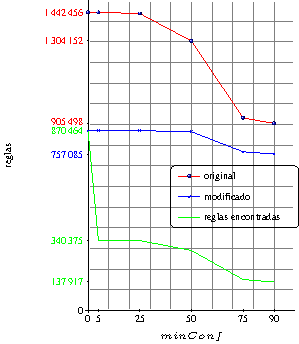
\includegraphics[width=.35\textwidth]{2-2-numReglas-foodmart.pdf}
  \hspace{.1\textwidth}
  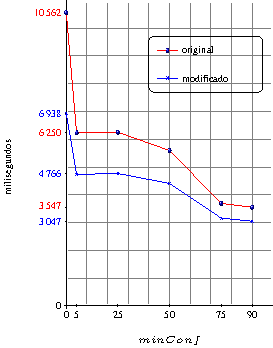
\includegraphics[width=.31\textwidth]{2-2-tiempo-foodmart.pdf}
  % \caption{Reglas analizadas (foodmart, $minSup = 0.005\%$)}
	\caption[\texttt{genrules()} original vs. nuestra modificación]{\footnotesize \texttt{genrules()} original vs. nuestra modificación (\texttt{foodmart}, $minSup=0.005\%$)}
	\label{fig:2-3-1-genrulesFoodmart}
\end{figure}


% \begin{wrapfigure}{o}{0.45\textwidth}
%   \centering
%   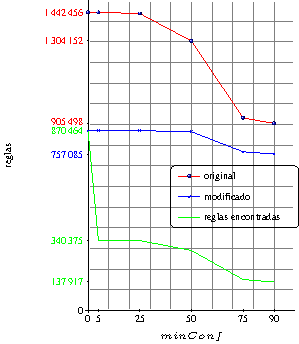
\includegraphics[width=.42\textwidth]{2-2-numReglas-foodmart.pdf}
%   % \caption{Reglas analizadas (foodmart, $minSup = 0.005\%$)}
%   \caption{\footnotesize Reglas analizadas (foodmart)}
%   \label{fig:2-3-1-numReglasFoodmart}
% \end{wrapfigure}
La primera observación a destacar de estos resultados es que la eficiencia de nuestro método depende de su implementación. Cuando no se impone un umbral de \confianza ($minConf = 0\%$) estamos obligando al algoritmo a mostrar todas las reglas existentes. En estas condiciones nuestro método analiza únicamente las reglas que contiene el almacén \D mientras que el método original analiza un 65.7\% más de las reglas encontradas en el análisis de \texttt{foodmart} y hasta un 13\,016.0\% más en el peor de los casos estudiados, al analizar \texttt{T40I10D100K} con \soporte mínimo del 0.5\%.




%TODO: Falta un valor, minSup = 0.1\%, minConf = 50\%
\begin{table}[htb]
   \scriptsize
   \begin{center}
      \begin{tabular}{cccccc} \hline
                     &          &        & \multicolumn{3}{c}{reglas} \\ \cline{4-6}
                     &          &        & \multicolumn{2}{c}{analizadas} & encontradas \\ \cline{4-5}
         fichero     & $minSup$ & $minConf$ & original   & modificado  & \\ \cline{1-1}\cline{2-2}\cline{3-3} \cline{4-4}\cline{5-5} \cline{6-6}
         T40I10D100K & 5\%      & 50\%   & 30            & 30          & 0 \\                      %Comprobado
         (Cálculos)  &          &        & ()            & ()          & \\
         Tiempo      &          &        & 0 msg         & 0 msg       & \\
                     & 1\%      & 50\%   & 5\,193\,340   & 398\,818    & 290\,273 \\
                     &          &        & (1\,789.1\%)  & (137.4\%)   & \\
                     &          &        & 30.3 sg       & 4.1 sg      & \\
                     &          & 0\%    & 5\,912\,979   & 401\,096    & 401\,096 \\
                     &          &        & (1\,474.2\%)  & (100\%)     & \\
                     &          &        & 30.3 sg       & 4.1 sg      & \\
                     & 0.5\%    & 50\%   & 606\,619\,662 & 6\,302\,454 & 4\,927\,893 \\
                     &          &        & (12\,309.9\%) & (127.9\%)   & \\
                     &          &        & 4\,772.7 sg   & 91.2 sg     & \\
                     &          & 0\%    & 846\,495\,481 & 6\,453\,924 & 6\,453\,924 \\
                     &          &        & (13\,116.0\%) & (100\%)     & \\
                     &          &        & 14\,266.6 sg  & 106.1 sg    & \\ \hline
      \end{tabular}
   \end{center}
   \caption{Reglas analizadas y encontradas (T40I10D100K)}
   \label{tab:T40I10D100K}
\end{table}



Al incrementar la \confianza mínima se analizan más reglas de las que finalmente serán aceptadas ya que muchas de ellas no superarán el umbral fijado. A pesar de que se acercan los valores obtenidos usando ambos algoritmos siempre se produce un gran ahorro al utilizar nuestra propuesta.

% En el almacén \texttt{T40I10D100K} peor de los casos analizamos con nuestra propuesta un 448\% más de las reglas existentes, correspondiendo a las reglas que no superan el umbral de \confianza fijado. El algoritmo original analiza en este caso un 556\% más de reglas.

Todo esto también se refleja en el tiempo de ejecución, notablemente inferior en todas las pruebas realizadas para el algoritmo modificado, hasta el extremo de tardar menos de 2 minutos en una ejecución en que el algoritmo original empleó más de 237 minutos (\texttt{T40I10D100K} con $minSup = 0.5\%$ y $minConf = 0\%$). Si aplicamos nuestra propuesta a las transacciones realizadas por un único usuario serán aún menores los tiempos, consiguiendo resultados en tiempo real para alimentar un \srw.









\subsection{Apriori2}
\label{sec:arm:ar:apriori2}
% !TEX root = ../../../Lazcorreta.Tesis.tex
% \ABIERTO%

Otra de nuestras propuestas consistió en crear un fichero similar a \D en el que sustituimos las \transacciones originales por el conjunto de \ars que satisface cada una de ellas. La idea original era aplicar \apriori a este nuevo conjunto, \R, para analizar a través de las reglas que cumple cada transacción "`cómo"' se comportan los usuarios que las generan en lugar de estudiar "`qué"' ítems relacionan los usuarios en una transacción.

\subsubsection{Reescribiendo \D para obtener \R}
Para estudiar el comportamiento de un usuario es preferible analizar qué reglas "`verifica"' en vez de centrar el análisis en los ítems que forman dichas regla. Supongamos que un usuario visita los lunes un \portalWeb solicitando las páginas $A$, $B$ y $C$ y un conjunto de páginas $P_1$. Los viernes este usuario visita las páginas $A$, $G$ y $H$ y un conjunto de páginas $P_2$. Supongamos también que las páginas de $P_1$ y $P_2$ no están relacionadas frecuentemente con la página $A$ y que nuestro sistema de recomendación no considera variables temporales por lo que no puede determinar si es lunes o viernes. Cuando el usuario entra en el \portalWeb y solicita la página $A$ es muy probable que le recomendemos visitar la página $B$ o $G$ si estamos usando los métodos tradicionales de recomendación. Si el usuario visita a continuación $G$ el sistema recomendará la página $H$, a continuación alguna de las páginas de $P_2$ y por último la página $B$ con menor probabilidad. De cualquier modo el hecho de que visite la página $A$ no es tan significativo como la posibilidad de usar las reglas de comportamiento ya guardadas en nuestro sistema (las reglas que contienen la relación entre los \kitemsets $AGH$ y $P_2$). Nuestro objetivo es aprovechar la capacidad que tenemos de analizar las reglas que se verifican en nuestro \portalWeb de forma independiente al número de páginas que contienen, proporcionar un método para medir la relación existente entre las reglas de comportamiento de nuestro \portalWeb y usando únicamente las transacciones proporcionadas por los usuarios.

Si estudiamos las reglas verificadas por cada transacción del repositorio original \D, podemos definir el conjunto de reglas \R que contiene una línea por cada transacción de \D conteniendo las reglas que verifica la transacción original. El objetivo de esta conversión, $\D\hookrightarrow\R$, es analizar en un segundo estudio las reglas que contiene \R utilizando el algoritmo \apriori.

Inicialmente esta tarea es simplemente exploratoria y se necesitan muchas horas para convertir el repositorio original \D en grandes repositorios \R con diferentes umbrales de \soporte y confianza. Los repositorios de reglas tienden a ser mucho más grandes que los de transacciones. Si una transacción verifica una regla que contiene un determinado \kitemset $l_k$ también verificará todas las reglas de los \itemsets contenidos en $l_k$. Por ejemplo, si la transacción $ABCD$ genera una regla también generará las cincuenta reglas que se deducen de sus subconjuntos:
\begin{itemize}
  \item 14 reglas de 4 ítems: $ABC\rightarrow D$, $ABD\rightarrow C$, \ldots $D\rightarrow ABC$
  \item 24 reglas de 3 ítems: $AB\rightarrow C$, $AB\rightarrow D$, \ldots $D\rightarrow BC$
  \item 12 reglas de 2 ítems: $A\rightarrow B$, $A\rightarrow C$ \ldots $D\rightarrow C$
\end{itemize}

Si usamos un umbral de confianza bajo, una transacción de \D con dos ítems generará una línea con 2 reglas en \R, una transacción con 3 ítems generará 12 reglas, una transacción con 4 ítems generará 50 reglas. \R crecerá exponencialmente en función de la longitud de las transacciones de \D.

El desmesurado tamaño de los repositorios \R obtenidos nos condujo a hacer un análisis exploratorio de las diferencias existentes entre \R y \D con el fin de reducir los datos que forman \R sin perder la información que contiene.




\subsubsection{Análisis descriptivo de las diferencias existentes entre \D y \R}
En la sección TAL se expuso una modificación del algoritmo de generación de reglas con la que se puede trabajar con umbrales de confianza muy pequeños. La razón por la que buscamos esta reducción, que en algunos casos consistía en la eliminación del umbral, se entiende mejor al revisar los resultados obtenidos, que se muestran en la figura~\ref{fig:2-1-DvsR} y el cuadro~\ref{tab:2-2-2-DvsR}. Conforme se reduce el valor de \confianza mínima se pierde información de las transacciones en estudio. Por ejemplo, al usar un \soporte mínimo del 5\% en el repositorio \texttt{T40I10D100K} las reglas obtenidas se derivan únicamente de un 32.6\% de las transacciones del repositorio, de lo que se deduce que más del 67\% de las transacciones originales son completamente ignoradas por el análisis.

%\afterpage{\clearpage}
\begin{figure}[htb]
   \centering
   \begin{subfigure}[b]{0.44\textwidth}
      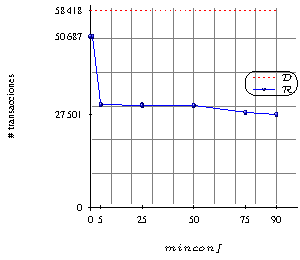
\includegraphics[width=\textwidth]{2-2-DvsR-foodmart-0_005.pdf}
      \caption{foodmart 0.005\%}
      \label{fig:2-1-foodmart0_005}
   \end{subfigure}%
   \hfill    
   \begin{subfigure}[b]{0.44\textwidth}
      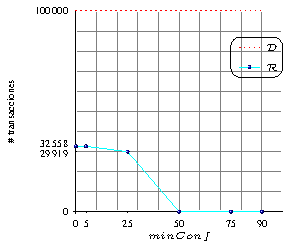
\includegraphics[width=\textwidth]{2-2-DvsR-T40I10D100K-5.pdf}
      \caption{T40I10D100K 5\%}
      \label{fig:2-1-T40I10D100K-5}
   \end{subfigure}
   \hfill
   \begin{subfigure}[b]{0.44\textwidth}
      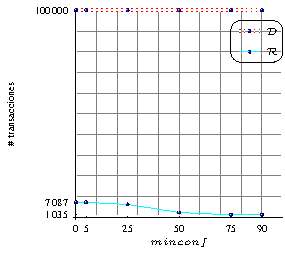
\includegraphics[width=\textwidth]{2-2-DvsR-T10I4D100K-1.pdf}
      \caption{T10I4D100K 1\%}
      \label{fig:2-1-T10I4D100K-1}
   \end{subfigure}
   \hfill    
   \begin{subfigure}[b]{0.44\textwidth}
      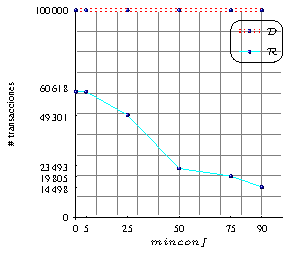
\includegraphics[width=\textwidth]{2-2-DvsR-T10I4D100K-0_5.pdf}
      \caption{T10I4D100K 0.5\%}
      \label{fig:2-1-T10I4D100K-0_5}
   \end{subfigure}
   \caption{\D vs \R}
\label{fig:2-1-DvsR}
\end{figure}

% \noindent
% \begin{table}[htb]
{\scriptsize
\begin{longtable}{cccccc}
   \caption{\D vs \R}\\
               &          &           & \multicolumn{2}{c}{transacciones} &            \\
   \hline
   fichero     & $minSup$ & $minConf$ &     \D      &        $\mathcal{R}$         & \D \'util \\ 
   \hline
\endfirsthead
   \multicolumn{6}{c}%
      {\tablename\ \thetable\ -- \textit{\ldots continuación}} \\
   \hline
               &          &           & \multicolumn{2}{c}{transacciones} &            \\ \cline{4-5}
   fichero     & $minSup$ & $minConf$ &     \D      &        $\mathcal{R}$         & \D \'util \\ 
   \hline
\endhead
\hline
\multicolumn{2}{r}{\textit{Continúa en la página siguiente\ldots}} \\
\endfoot
\hline
\endlastfoot
\centering
  foodmart & 0.005\% & 90\% & 58\,418  & 27\,501 & 47.1\% \\
           &         & 75\% &          & 28\,125 & 48.1\% \\
           &         & 50\% &          & 30\,201 & 51.7\% \\
           &         & 25\% &          & 30\,212 & 51.7\% \\
           &         & 5\%  &          & 30\,440 & 52.1\% \\
           &         & 1\%  &          & 50\,687 & 86.8\% \\
           &         & 0\%  &          & 50\,687 & 86.8.\% \\
   \hline
  T40I10D100K & 5\% & 50\% & 100\,000  & 0       & 0\%     \\         %Comprobado
				  &     & 25\% &           & 29\,919 & 29.9\%  \\         %Comprobado
              &     &  5\% &           & 32\,558 & 32.6\%  \\         %Comprobado
              &     &  0\% &           & 32\,558 & 32.6\%  \\         %Comprobado
              & 1\% & 50\% &           & 92\,227 & 92.2\%  \\         %Comprobado
				  &     & 25\% &           & 99\,956 & 100.0\% \\         %Comprobado
				  &     &  5\% &           & 99\,956 & 100.0\% \\
				  &     &  1\% &           & 99\,956 & 100.0\% \\
				  &     &  0\% &           & 99\,956 & 100.0\% \\
				      & 0.5\% &  50\% &        & 99\,835 & 99.8\% \\          %Comprobado
              % &     & 25\% &           & \, & \% \\
              % &     &  5\% &           & \, & .\% \\
              % &     &  1\% &           & \, & .\% \\
              % &     &  0\% &        & \, & .\% \\
              % & 0.1\% &  50\% &        & \, & .\% \\
              % &     & 25\% &           & \, & .\% \\
              % &     &  5\% &           & \, & .\% \\
              % &     &  1\% &           & \, & .\% \\
              % &     &  0\% &        & \, & .\% \\
   \hline
  T10I4D100K & 5\%   & 50\%  & 100\,000  & 0       & 0\%    \\
	           &       & 25\%  &           & 15\,475 & 15.5\% \\
             &       & 5\%   &           & 32\,558 & 32.6\% \\
             & 1\%   & 50\%  &           &  2\,211 &  2.2\% \\
			       &       & 25\%  &           &  6\,109 &  6.1\% \\
				     &       &  5\%  &           &  7\,087 &  7.1\% \\
				     &       &  1\%  &           &  7\,087 &  7.1\% \\
				     &       &  0\%  &           &  7\,087 &  7.1\% \\
				     & 0.5\% &  50\% &           & 23\,493 & 23.5\% \\
				     &       & 25\%  &           & 49\,301 & 49.3\% \\       %Comprobado
				     &       &  5\%  &           & 60\,618 & 60.6\% \\
				     &       &  1\%  &           & 60\,618 & 60.6\% \\
				     &       &  0\%  &           & 60\,618 & 60.6\% \\
             % & 0.1\% &  50\% &        & \, & .\% \\
             % &     & 25\% &           & \, & .\% \\
             % &     &  5\% &           & \, & .\% \\
             % &     &  1\% &           & \, & .\% \\
             % &     &  0\% &        & \, & .\%
\label{tab:2-2-2-DvsR}
\end{longtable}
}


Existen muchas aproximaciones en el estado del arte que buscan la reducción de las dimensiones del problema a tratar utilizando técnicas estadísticas basadas en la frecuencia de los ítems, sin embargo no se tienen en cuenta ciertos detalles, como el hecho de que los resultados son sólo significativos para un reducido grupo de individuos de la población en estudio.

En este trabajo usamos valores para el \soporte y \confianza mínimos que puedan ser utilizados en ordenadores personales convencionales sin generar problemas de falta de recursos, de modo que podamos atender al mayor número de individuos de la población en estudio. El tamaño de los repositorios \R obtenidos con estos parámetros es tan grande que no podemos analizarlos directamente por lo que proponemos un nuevo algoritmo para dividir \R en diferentes repositorios que puedan ser analizados convenientemente.



\subsubsection{División automática del repositorio de reglas}
Existen muchas investigaciones proponiendo métodos para dividir los repositorios originales de transacciones, pero todos ellos se basan en un alto control y \clasificacion del conjunto de ítems disponibles en el sistema. Nuestra propuesta no usa esta información adicional porque se obtiene de una gestión del sistema y no de del propio uso del mismo. Definimos un conjunto de familias de reglas para dividir el repositorio \R y agrupar aquellas reglas que los usuarios relacionan entre sí cuando interactúan con el sistema. A continuación se describe el algoritmo que proponemos.

\begin{enumerate}
  \item Seleccionar la regla con mayor \soporte, en caso de empate seleccionar la regla con mayor confianza y en caso de empate seleccionar la regla que contenga más ítems.
  $$R_1 = max_i\{soporte(R_i)\} \wedge$$
  $$\left(confianza(R_1) = max_j\{confianza(R_j) | soporte(R_j) = soporte(R_1)\} \right)$$
  Esta regla será el elemento principal de la primera familia de reglas, $\mathcal{F}_1$.
  \item Dividir \R en subconjuntos de reglas. El primer repositorio, $\R_1$, contendrá todas las líneas de \R que tengan la regla $R_1$ y el segundo repositorio, $\R_\infty$, contendrá el resto de líneas de \R.
  \item Ejecutar el algoritmo \apriori sobre $\R_1$ y aplicar de nuevo el paso 1 para seleccionar $R_2$, la regla de $\R_1$ que aparece con mayor frecuencia junto a $R_1$.
  \item Comprobar el \soporte de $R_2$ en $\R_\infty$: si el \soporte de $R_2$ en $\R_1$ es mayor que su \soporte en $\R_\infty$ se añade $R_2$ a la familia $\mathcal{F}_1$; en otro caso se elimina $R_2$ de $\R_1$.
  \item Volver al paso (3) mientras queden reglas no clasificadas en $\R_1$.
\end{enumerate}

Cuando se ha completado la definición de la primera familia de reglas se eliminan todas las reglas pertenecientes a $\mathcal{F}_1$ del repositorio original de reglas, \R, y las transacciones que queden vacías. A continuación se utiliza el mismo procedimiento para generar $\mathcal{F}_2$, la segunda familia de reglas. El algoritmo finaliza cuando $\R_\infty$ no contiene reglas asociadas, es decir, cuando todas las transacciones de $\R_\infty$ contienen únicamente una regla.



\subsubsection{Propuesta de sistema de recomendación}
Hemos definido un \sr en el que aplicar la modificación en dos pasos del algoritmo \apriori. El objetivo principal es obtener recomendaciones personalizadas para los usuarios de nuestro portal de educación, generando recomendaciones en tiempo real en forma de enlaces. El proceso se define a continuación:

\begin{enumerate}
  \item Un usuario entra en el sistema y selecciona el ítem $A$.
  \item El sistema sólo puede usar la información almacenada sobre los ítems directamente relacionados con $A$, es decir, las reglas originales cuyo antecedente es $A$ -- esta es la recomendación clásica basada en \ARs. La primera recomendación se basa únicamente en fecuencias (el sistema recomendará los consecuentes de las reglas con mayor \confianza que tengan al ítem $A$ como antecedente).
  \item El usuario selecciona un segundo ítem, $B$.
  \item A partir de ahora podemos usar la nueva información que hemos recogido sobre el comportamiento de la población de usuarios, las reglas que verifican en su visita a nuestro \portalWeb. Obtenemos las reglas derivadas del \kitemset $l_k$ y buscamos la familia a la que pertenecen, $\mathcal{F}_i$.
  \begin{itemize}
    \item Si $\mathcal{F}_i$ contiene reglas derivadas de las reglas verificadas por el usuario en esta visita, entonces hay una \confianza del 100\% entre las reglas descubiertas y las reglas verificadas por el usuario. En este caso el sistema recomendará los ítems de las reglas descubiertas con mayor \soporte. A diferencia de los métodos clásicos, esta propuesta descubre reglas que no tienen los ítems visitados por el usuario como antecedentes; esto es importante ya que el análisis realizado ignora por completo el orden de selección de los ítems.
    \item Si $\mathcal{F}_i$ no contiene reglas derivadas se usarán las reglas con mayor \confianza (y mayor \soporte en caso de empate) en relación con las reglas verificadas por el usuario. Adicionalmente, para resolver el problema de encontrar recomendaciones basadas en el antecedente, es posible encontrar reglas con cualquier ítem seleccionado por el usuario. Esto no puede llevarse a cabo con el método clásico.
  \end{itemize}
  \item El usuario selecciona un tercer ítem, $C$.
  \item Repetimos el tercer paso buscando una o más familias que contengan las reglas derivadas del \kitemset $l_k = \{A,B,C\}$.
\end{enumerate}

Esta aproximación conduce a una nueva experiencia con nuestro sistema educacional. Los usuarios se pueden sentir más confortables en su interacción con el sistema ya que pueden llevar a cabo sus tareas más rápidamente cuando utilizan los enlaces recomendados por el sistema.




% \subsection{Experimentación}
% \label{sec:2-2-X-Experimentacion}
% \input{./2-ARM/2-3-GeneracionDeAR/2-3-X-Experimentacion}
